\documentclass{school-22.101-notes}
\date{November 14, 2011}

\begin{document}
\maketitle

\subtopic{Contributors of Binding Energy}
Next we are going to talk about the contributions to the binding energy: Volume Effect (positive effect), Surface Effect (negative effect because less nucleon interaction on the surface), Coulomb Interaction (negative effect), Asymmetry Effect (negative effect), Parity Effect (can be positive, negative, or no effect). 
\begin{enumerate}
    \item Volume Contribution: An initial guess is that, each nucleon would interact with any other nucleon (A-1 of them); so together the volume contribution is proportional to $A(A-1) \approx A^2$. This is not quite right because nuclear interactions are short range (strong nuclear force). Assume that each nucleon has about the same number of neighbors (except on the surface -- surface effect would take into account this part), hence the volume term should be roughly proportional to $A$:
    \eqn{B_V = 15.5 \MeV A} 

    \item Surface Contribution: Surface nucleons are surrounded by less neighbors than the bulk (inner) nucleons. The surface nucleons do not contribute to B as much, hence we need to subtract from the binding energy a term proportional to the surface area, which is 2/3 power of the volume (or, say A). Experimental data tells us $a_S \approx a_V$ as expected. 
    \eqn{B_S = - 16.8 \MeV A^{2/3}}

    \item Coulomb Contribution: the coulomb repulsion of protons make nucleus less tightly bound. For a total charge is $Ze$, we consider a constant charge distribution $\rho = \frac{Ze}{\frac{4\pi}{3} R^3}.$ If we consider a small shell from $r$ to $r + \dr$, then the Coulomb force between the spherical core and the shell is 
    \eqn{ \int_0^{R} \frac{1}{r} \underbrace{\left( \frac{4}{3} \pi r^3 \rho \right)}_{\mathrm{core}} \underbrace{\left(\rho \cdot 4 \pi r^2 \dr \right)}_{\mathrm{shell}} = \frac{3}{5} \frac{Z^2 e^2}{R}.}
    Then we have to correct the term by taking into account the `self-energy' of each proton with the magnitude of $\frac{3e^2}{5R}$ (this term arises from that we assume the charges of protons `smeared' over the entire nucleus, hence under this assumption each proton would repel itself as well), so the result is ($r_0 = 1.2 \fm$):
    \eqn{V_{coul} = \frac{3}{5} \frac{Z(Z-1)e^2}{R} = \frac{3}{5} \frac{Z(Z-1) e^2}{r_0 A^{1/3}} = 0.72\MeV \frac{Z(Z-1)}{A^{1/3}} }

    \item Asymmetry Contribution: this term arises when number of protons does not equal number of neutrons. To start, we notice there is no isotope that has way more neutrons than protons. Typically, 
    \begin{align}
    \begin{dcases*}
    Z \sim 0.4 N & Large A \\
    Z \sim N & Small A
    \end{dcases*}
    \end{align}
    \begin{enumerate}
    \item At small A, $N \sim Z$ because it is favored. When $N \neq Z$, there is an effect that make nucleus less stable, reflected as a decrease in the binding energy which puts the nucleus at a higher energy. 
    \item At larger A, Coulomb term wins Asymmetry term, hence favoring more neutrons than protons. Let us consider the difference between an equal-level n \& p configuration and a non-equal one. Starting from an equal configuration, we need to convert $\frac{N-Z}{2}$ number of protons to neutrons. Assume $\Delta$ is the energy difference between two states, then the energy penalty for EACH proton to go above the last occupied neutron level is: $\Delta \frac{N-Z}{2}$. For all $\frac{N-Z}{2}$ protons, the total energy penalty is $\Delta \left( \frac{N-Z}{2} \right)^2$. We approximate $\Delta$ from filling the potential well $V_0$ uniformly with $\frac{A}{2}$ nucleons: 
    \eqn{\frac{A}{2} \Delta = V_0 \Rightarrow \Delta \sim \frac{50 \fsp \MeV}{A/2} }
    Then the asymmetry term is:
    \eqn{\Delta E_{\mathrm{sym}} = 23 \MeV \frac{(N-Z)^2}{A} }
    \end{enumerate}

    \item Parity Contribution: this term arises from the tendency of the like nucleons (neutron \& neutrons, protons \& protons) to couple pairwise to more stable configurations.
    \begin{enumerate}
    \item Odd N, odd Z: weakly bound, lose binding energy, $\sim -a_p A^{-3/4}$;
    \item Odd A: no effect;
    \item Even N, even Z: tightly bound, gain binding energy, $\sim a_p A^{-3/4}$.
    \end{enumerate}

    \item Summary: Together, Binding energy is:
    \eqn{B = \underbrace{15.5 A - 16.8 A^{2/3} - 0.72 \frac{Z(Z-1)}{A^{1/1}}}_{\mbox{`liquid-drop model,' collective behavior.}} \underbrace{- 23 \frac{(A-2Z)^2}{A} \pm 34 A^{-3/4}}_{\mbox{`shell model,' individual nucleon behavior.}}   }
    In Figure~\ref{binding-effect}, the peak at around $A = 60$ is a result of the surface effect and the Coulomb effect. 
    \begin{figure}
        \centering
        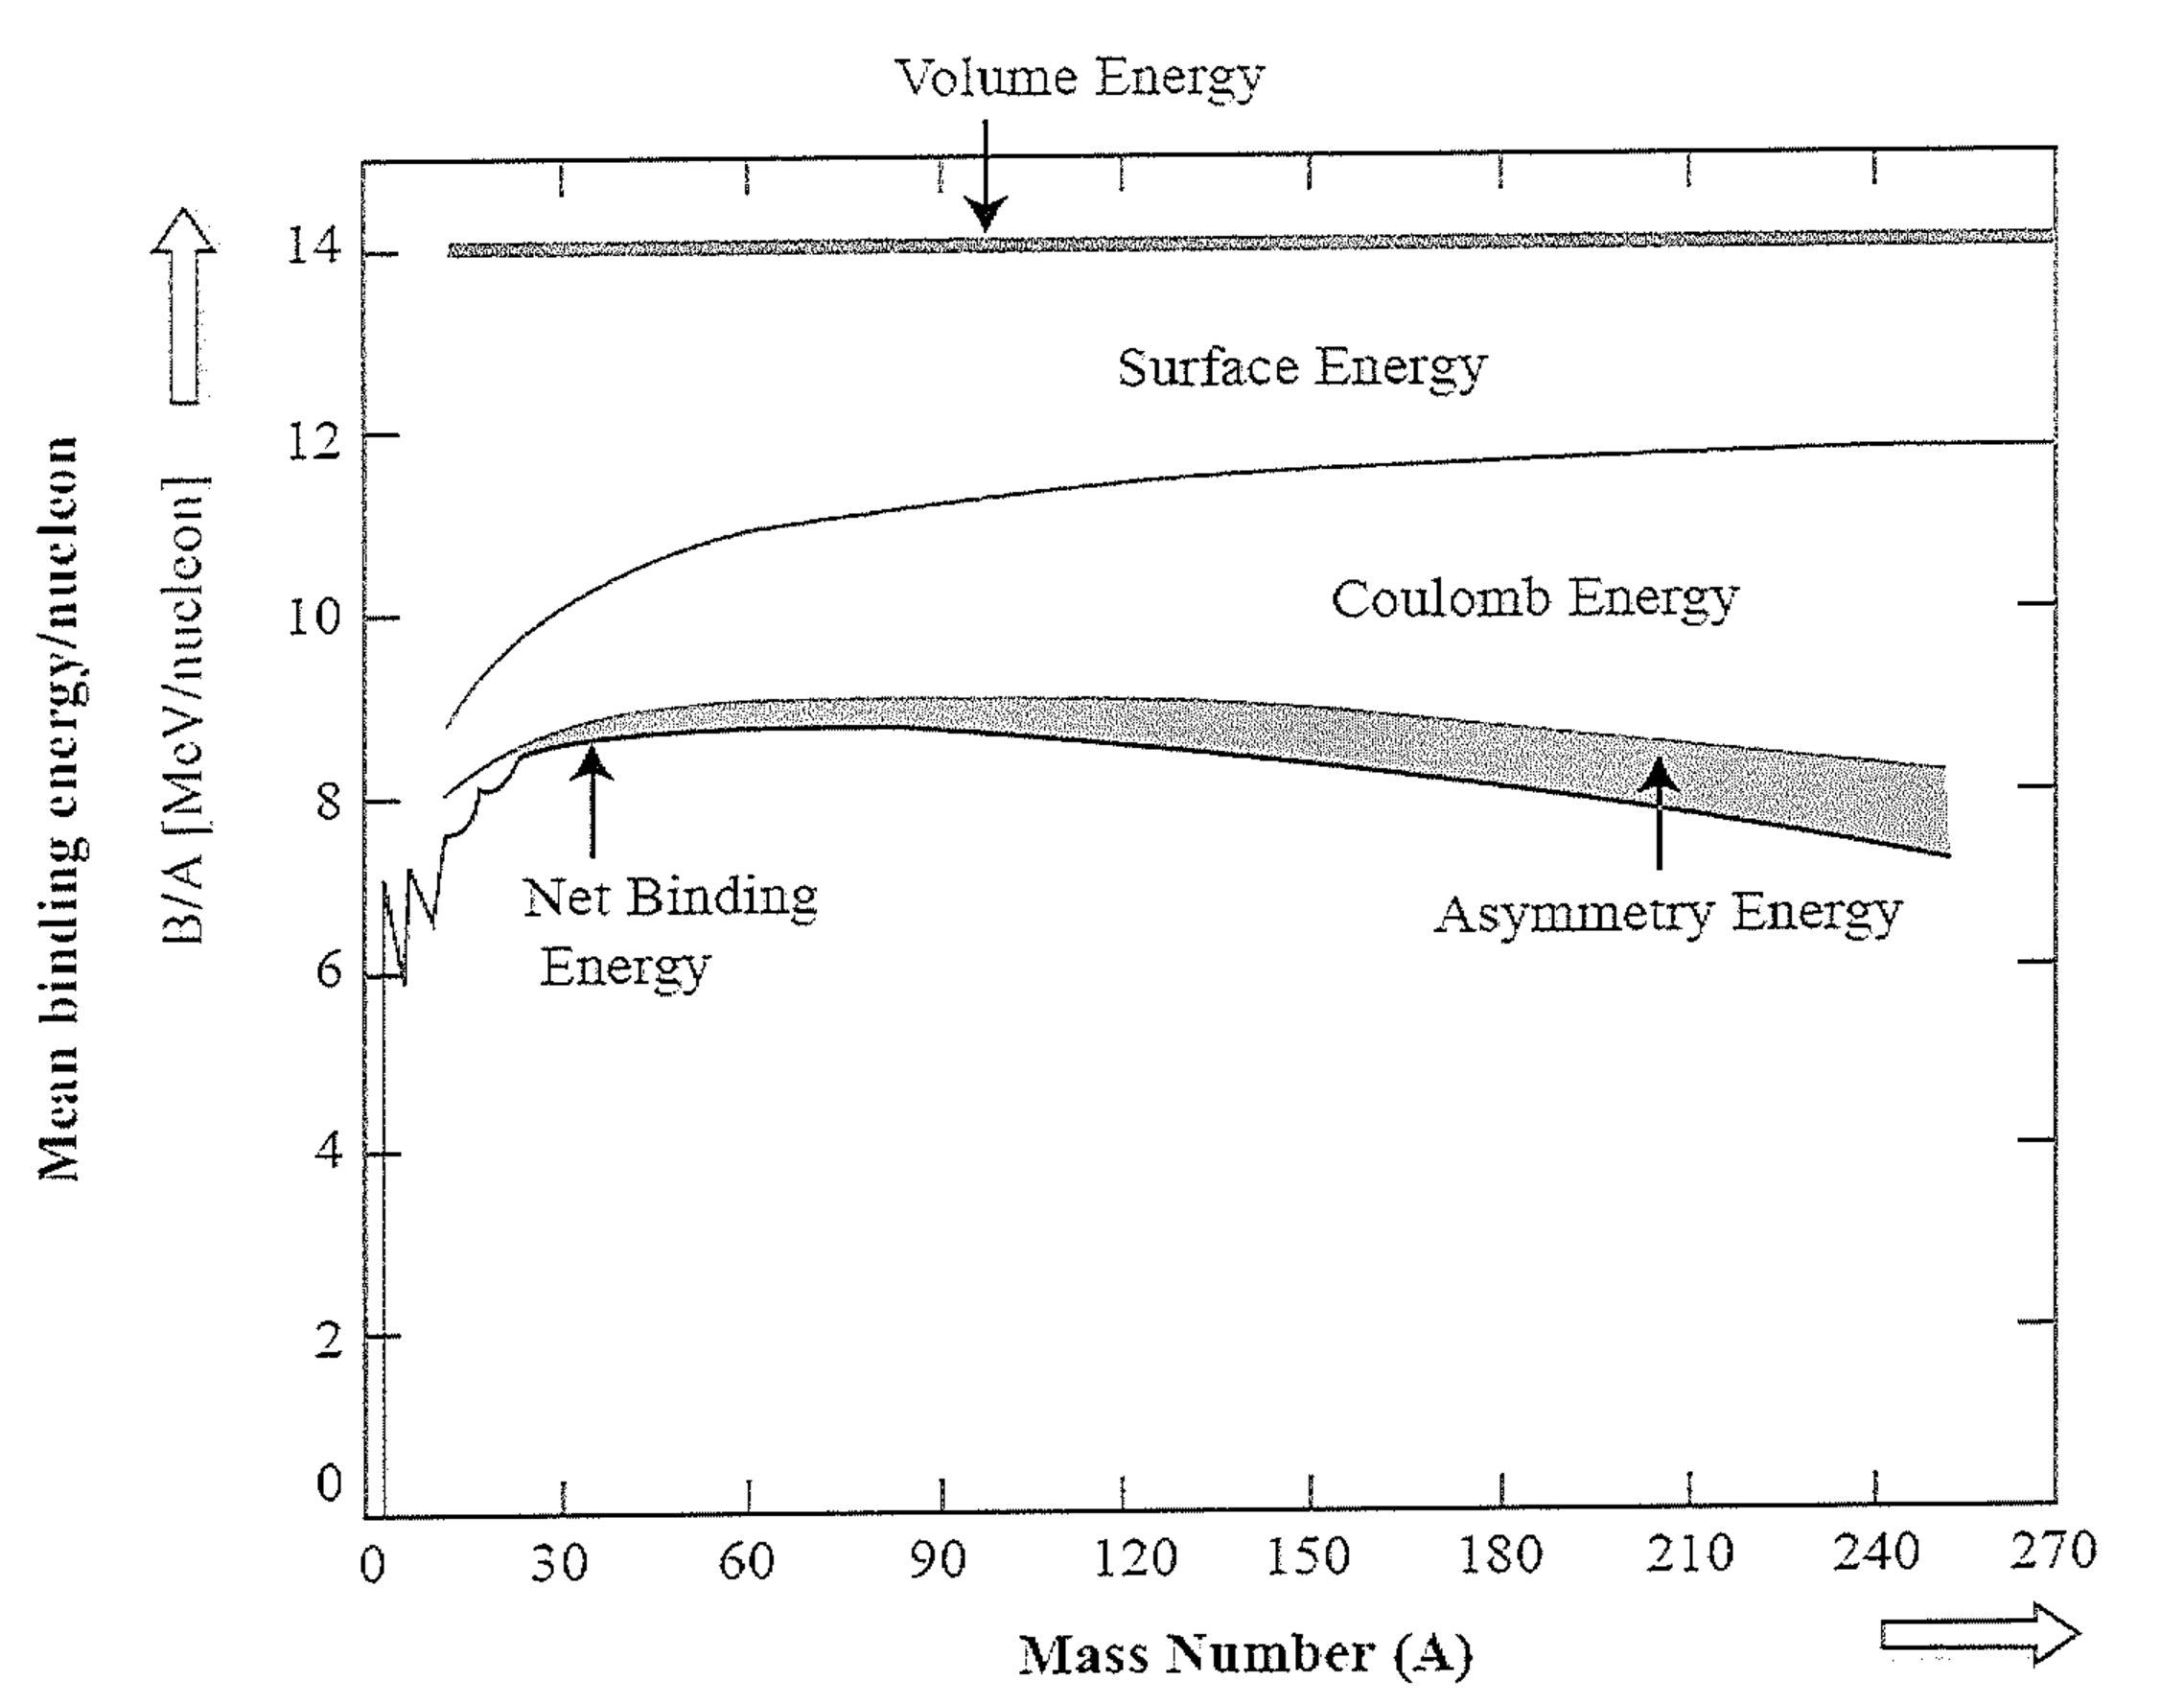
\includegraphics[width=4in]{images/rd/binding-effect.png}
        \caption{Relative Contributions to the Binding Energy Per Nucleon Showing the Importance of the Various Terms in te Semi-empirical Weizacker Formula \label{binding-effect}}
    \end{figure}
\end{enumerate}


\topic{Semi-Empirical Mass Formula (SEMF): Mass Parabolas, Stability}
Now that we have found the binding energy, we can write an expression for the mass. The mass formula comes out to be \textbf{parabola}, and the minimum mass corresponds to stability\footnote{This is an important point: notice in Eq.~\ref{BAZ}, the smaller the mass, the larger the binding energy, and binding energy is a negative term, so the smaller the total energy, the more stable. }.
\begin{align}
B(A,Z) &= \left[ Z m_H + N m_n - m(A,Z) \right] c^2  \label{BAZ}\\
m(A,Z) c^2 &= \left[ Z m_H + N m_n \right] c^2 - B(A,Z) = Z^2 (\cdots) + Z(\cdots) + C 
\end{align}
That is to say, for a given A, $m(Z)$ is a parabola, then there exists a $Z$ such that $m(Z)$ is minimum, and this is the most stable one. Of course this is a simple approximation that does not take into account stuffs like paring effect yet. 

If we take the derivative of the $m(A,Z)$ equation and set it to zero, we find $Z_{\mathrm{min}}$ to be: 
\eqn{ Z_{\mathrm{min}} \approx \frac{A/2}{1 + \frac{1}{4} \frac{a_c}{a_{\mathrm{sym}}} A^{3/4}} }
At small A, $Z_{\mathrm{min}} \sim \frac{A}{2}$. At large A, $Z_{\mathrm{min}} < \frac{A}{2} \sim 0.41 A$. 

Back to mass parabola, at $Z > Z_{\mathrm{min}}$, there are too many protons; $Z < Z_{\mathrm{min}}$, there are too many neutrons. By nature these nuclei want to undergo decay to reach stability (see Figure~\ref{A135} and Figure~\ref{A102}). 
\begin{enumerate}
\item Proton-rich nuclei go through $\beta^+$ decays: \ce{p^+ \to n + \beta^+ + \gamma}, or Electron Capture (E.C.): \ce{p + e^- \to n + \gamma}. Example: \ce{^{16}_9 F_7 \to ^{16}_8 O_8 + \beta^+ + \gamma}. 
\item Neutron-rich nuclei go through $\beta^-$ decays: \ce{n \to p + \beta^- + \gamma}. Example: \ce{^{16}_7 N_9 \to ^{16}_8 O_8 + \beta^- + \gamma}.
\item For a decay process to happen, it has to be \textcolor{blue}{energetically allowed, $M_{\mathrm{final}} < M_{\mathrm{initial}}$, that is, goes down on the M vs. Z curve.}
\end{enumerate}
\begin{figure}
  \centering
  \subfloat[A=135]{\label{A135}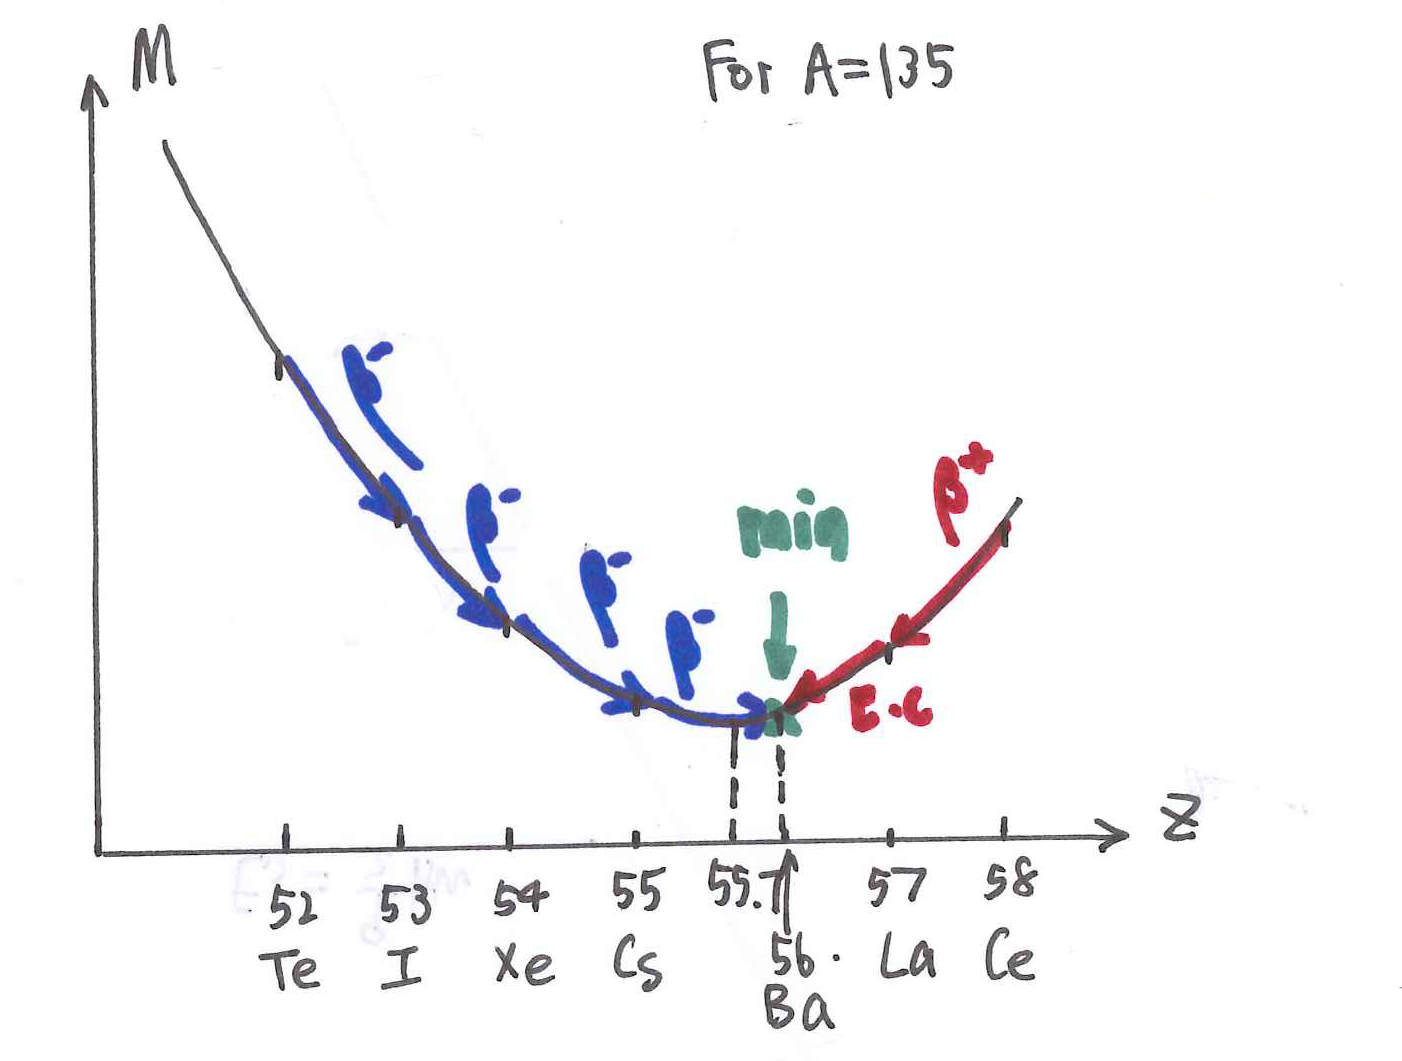
\includegraphics[width=0.4\textwidth]{images/rd/M-Z-A135.png}}                
  \subfloat[A=102]{\label{A102}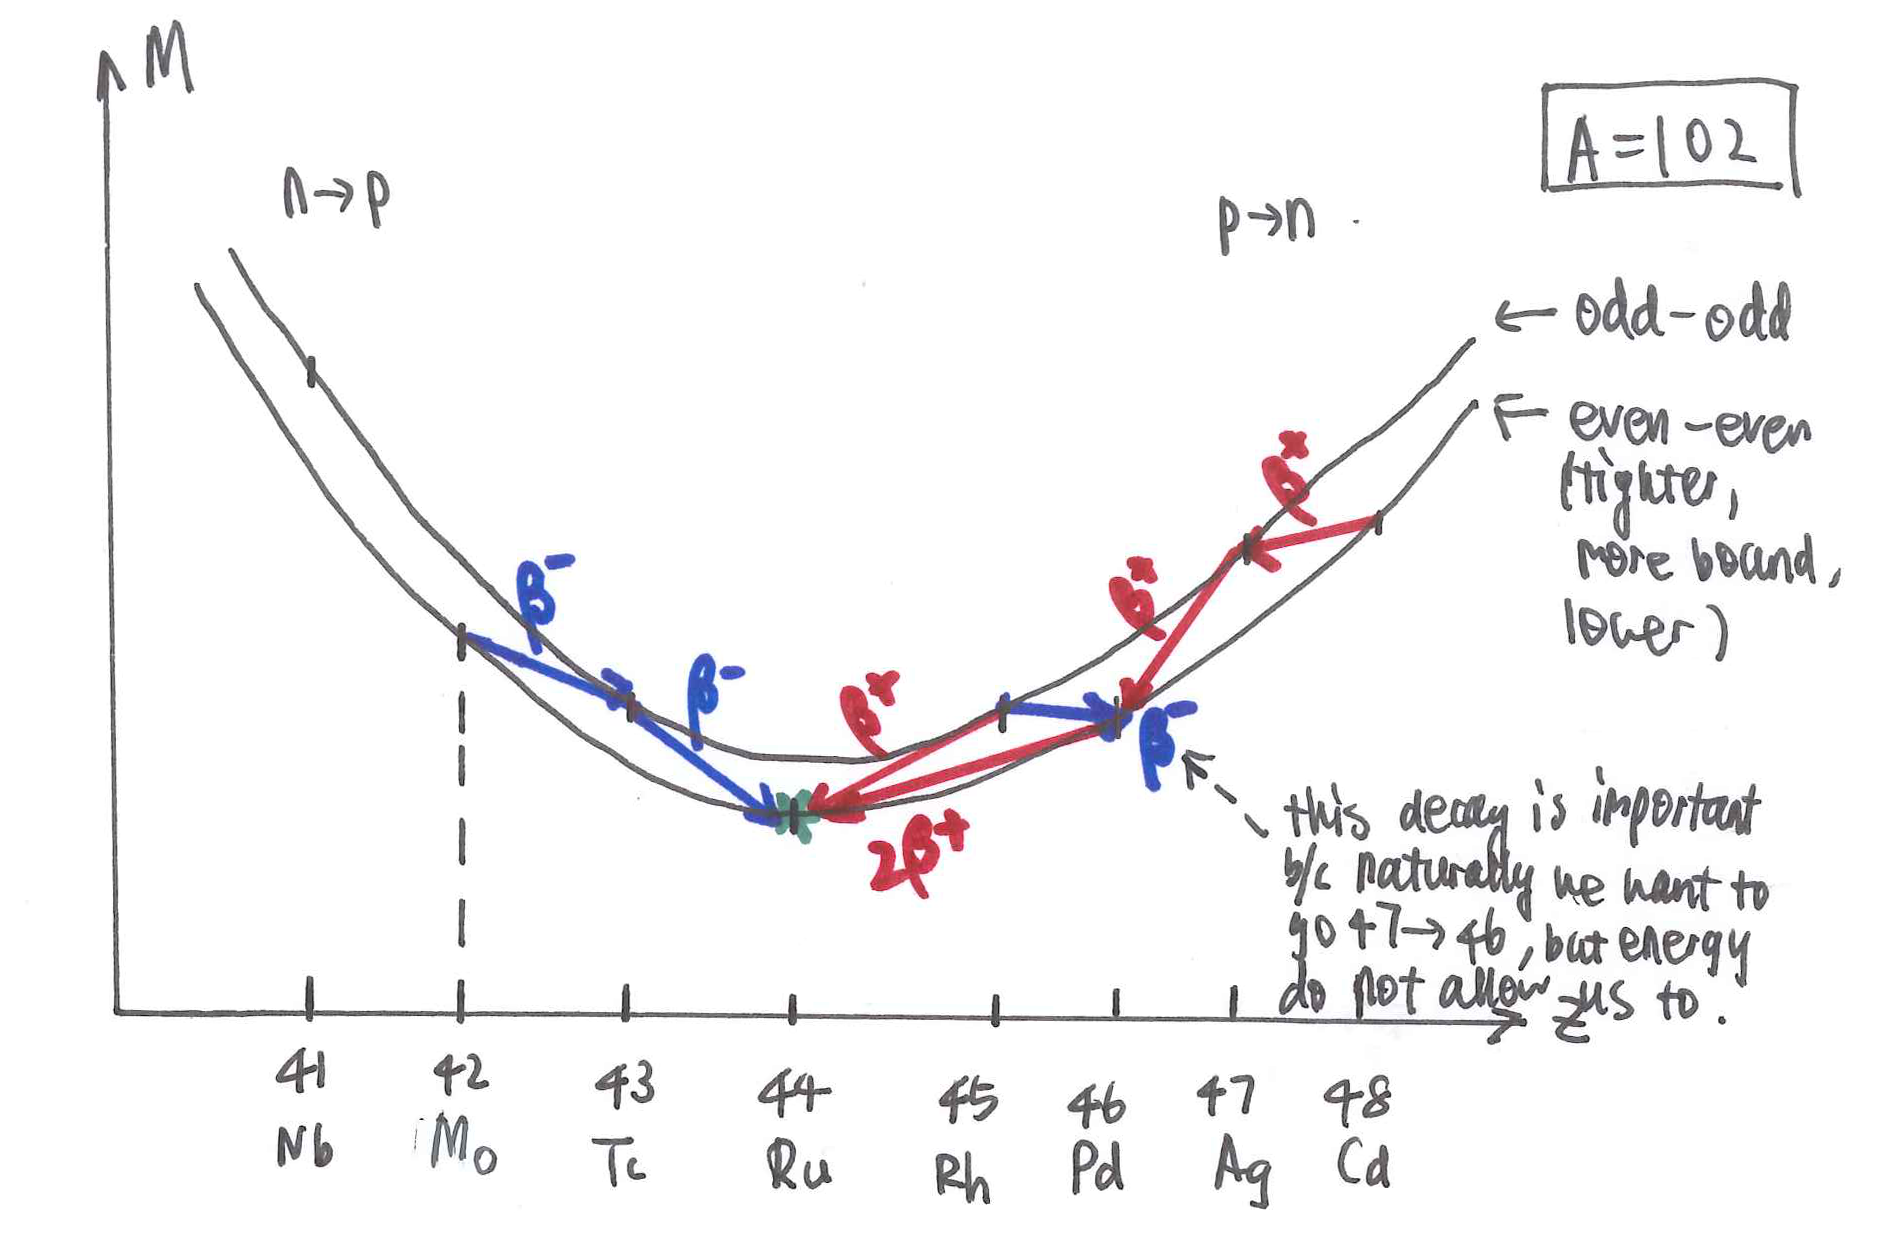
\includegraphics[width=0.6\textwidth]{images/rd/M-Z-A102.png}}
  \caption{Mass Parabola, Two Examples}
\end{figure}
\end{document}
